\documentclass[conference]{IEEEtran}
%\IEEEoverridecommandlockouts
% The preceding line is only needed to identify funding in the first footnote. If that is unneeded, please comment it out.
\usepackage{cite}
\usepackage{amsmath,amssymb,amsfonts}
\usepackage{algorithmic}
\usepackage{graphicx}
\usepackage{textcomp}
\usepackage{xcolor}

\usepackage{url}
\usepackage{hyperref}

\usepackage{tabularray}

%\def\BibTeX{{\rm B\kern-.05em{\sc i\kern-.025em b}\kern-.08em
%    T\kern-.1667em\lower.7ex\hbox{E}\kern-.125emX}}
\begin{document}

\title{A novel compression approach for time series monitoring data\\}

\author{\IEEEauthorblockN{1\textsuperscript{st} Carlos Rolo}
\IEEEauthorblockA{\textit{Instaclustr} \\
\textit{Netapp}\\
Lisbon, Portugal \\
carlos.rolo@netapp.com}
\and
\IEEEauthorblockN{2\textsuperscript{nd} Ben Bromhead}
\IEEEauthorblockA{\textit{Instaclustr} \\
\textit{NetApp}\\
Christchurch, New Zealand \\
ben.bromhead@netapp.com}
\and
\IEEEauthorblockN{3\textsuperscript{hd} Joshua Varghese}
\IEEEauthorblockA{\textit{dept. name of organization} \\
\textit{Open SI(NetApp)}\\
Canberra, Australia \\
u3227463@uni.canberra.edu.au}
}

\maketitle

\begin{abstract}
    This study introduces a novel approach to time series compression tailored for the complexities of computer systems monitoring.
    The Advanced Time Series Compression (ATSC) methodology, drawing inspiration from established audio compression techniques, achieves significant compression ratios. It enables storing time series data using 880 times less space than its original uncrompressed format and approximately an order of magnitude less than state-of-the-art open-source compression methods.
    The data representation of a time series is converted from a sequence of points (time and the measured value) to a mathematical formula (and its parameters) by using dynamicly sized blocks of consecutive points to split the series and applying mathematical modeling to each block of points.
    Selection of the mathematical formula is based on information retrieved from the time series and optimised to fit for desired maximum compression and error rates.
    The time component of the time series is reduced to a simple index that keeps the representation of time for each point and allows the precise retrieval and efficient streaming of data segments. 
    ATSC presents a promising solution for efficiently managing high sample rate time series data within the realm of computer systems monitoring.
    Here, we present promising results from initial testing against known open source state-of-the-art compression systems. 
\end{abstract}
\vspace{5pt}
\begin{IEEEkeywords}
Time Series Compression, Function Approximation, Data Storage, Streaming, Indexing, Computer Systems Monitoring
\end{IEEEkeywords}

\section{Introduction}
% Present your research topic
In this study we introduce a novel method to compress time series monitoring data\cite{influx}. 
Our approach enabled compression ratios of up to 3000x in test scenarios and up to 880x with real-world production data.
% Capture reader interest
Current computer systems monitoring data is lossy by nature, as it is generally sampled, and as such, not capturing all events. The sampling rate can be varied, ranging from 1 sample per second to a sample per minute\cite{monitoring-samples}, or even more\cite{microsoft}.
% Define your specific research problem and problem statement
Capturing and storing monitoring data can take massive amounts of space. In our test case, a group of 57 servers running the Apache Cassandra database generated 600 MB in less than a day.
Thus, monitoring data can be a significant burden in terms of storage and computational resources. Additionally, viewing data stored in the cloud incurs extra costs from egressing data.
% Summarize existing research
Current approaches tackle these problems by compressing time series data using several generic and/or specific algorithms\cite{timescale}\cite{dzone}\cite{compression} (e.g. Gorilla\cite{gorilla}).
Domain-specific research for time series compression\cite{nasa-compression}\cite{smartgrid} and improvements to existing algorithms\cite{victoria} have been performed.
Our approach leverages signal processing-specific knowledge from the multimedia domain (e.g., from FLAC\cite{flac}), starting with the premise that monitoring data is inherently lossy..
% Highlight the novelty and contributions of the study
We treat data as signals and leverage previously established signal processing techniques (e.g., Fast Fourier Transform (FFTs) and splines\ref{math_aprox}) to approximate data points using mathematical formulas at the cost of precision.
Using an approach that shares similarities with those used in domains such as audio compression, we developed a time-series compressor capable of very high compression ratios, and fast decompression and streaming capabilities.

\begin{figure}[ht]
  \centering
  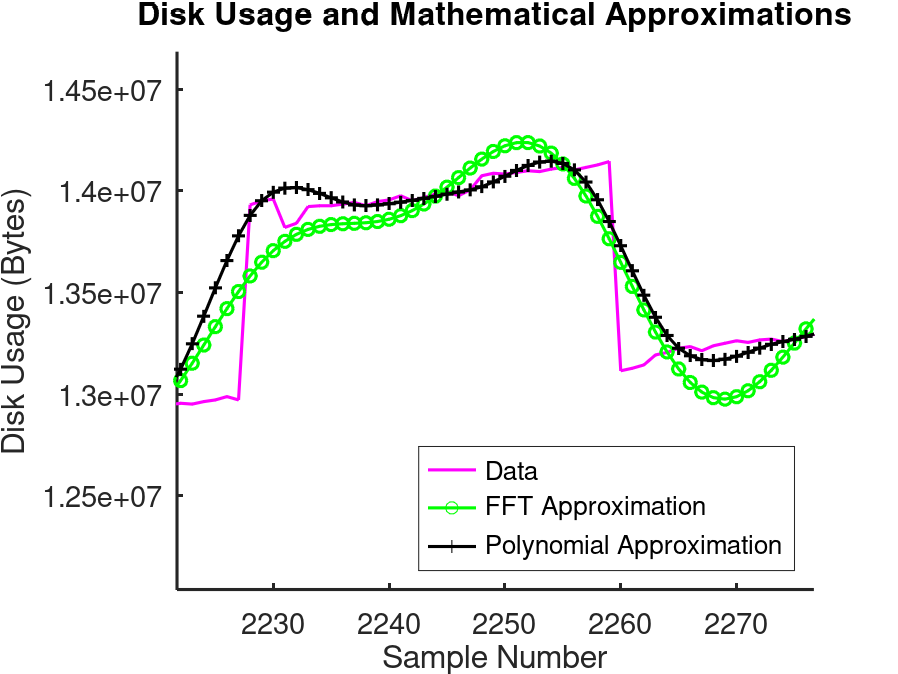
\includegraphics[width=0.5\textwidth]{math_approximation-4.png}
  \caption{A disk usage metric approximated by a Fast Fourier Transform and a Catmull-Rom interpolation.}
  \label{math_aprox}
\end{figure}

Prior to the mathematical modelling of the signal, the data is split into blocks with a dynamic size.
This is complemented by an indexing technique that allows the streaming of data without its complete decompression.
The compressor can either operate in lossy or lossless mode. Importantly, even when operating in a lossy manner, the shape of the time series is preserved.
The compression ratios achieved using our method enables avoiding data aggregation techniques (such as roll-ups, averaging points over larger time spans, and other summary based techniques) and culminate in storage and compute savings.
% Give an overview of the paper’s structure
In the following sections, we discuss the context leading to our research while exploring the architecture of our compressor and providing a detailed explanation of its dynamic blocking, modelling, and indexing aspects. Furthermore, we expand on the topic of error correction for minimizing compression artifacts and discuss the results obtained with this approach on production datasets.

\section{Background}

In the dynamic landscape of computer systems monitoring, the impetus for our research stems from critical challenges that impact the efficiency and cost-effectiveness of current practices\cite{10.1007/978-3-319-63712-9_8}. 

\subsection{High Storage Cost}

The exponential growth of data in computer systems monitoring has led to soaring storage costs.
Traditional methods often struggle to cope with the sheer volume of information generated by processes, databases, and overall system health monitoring.
Our research delves into innovative time-series compression techniques that alleviate the burden of high storage costs, offering a sustainable solution for data retention and management. 

\subsection{Balancing Data Reduction and Information Preservation}
Conventional practices often resort to techniques such as averaging, sub-sampling or undersampling to manage the overwhelming data volumes. This approach effectively reduces the amount of data points but is undermined by the loss of valuable information.
Our research addresses this trade-off by proposing advanced time-series compression methods that achieve data reduction without sacrificing critical insights and information\ref{fft_comparison}. 

\subsection{Computational Challenges in Traditional Monitoring Techniques}
Traditional approaches, such as point-walking algorithms, demand substantial computational resources to process vast amounts of monitoring data\cite{10.14778/2735479.2735481}. Recognizing the strain on computing capabilities, our method introduces a more resource-efficient paradigm by exploring novel compression techniques inspired by audio processing.

Our comprehensive approach tackles the immediate challenges of high storage and egress costs while addressing the inherent trade-offs of data reduction techniques. The overarching goal is to improve the landscape of computer systems monitoring by introducing a cost-effective and information-rich paradigm through advanced time-series compression.  

\section{Architecture}

In this section we describe the internals of the ATSC compressor. That includes both compressor\ref{internal} and decompressor, also internal structures and any other auxiliary mechanisms used.

\begin{figure}[h]
  \centering
  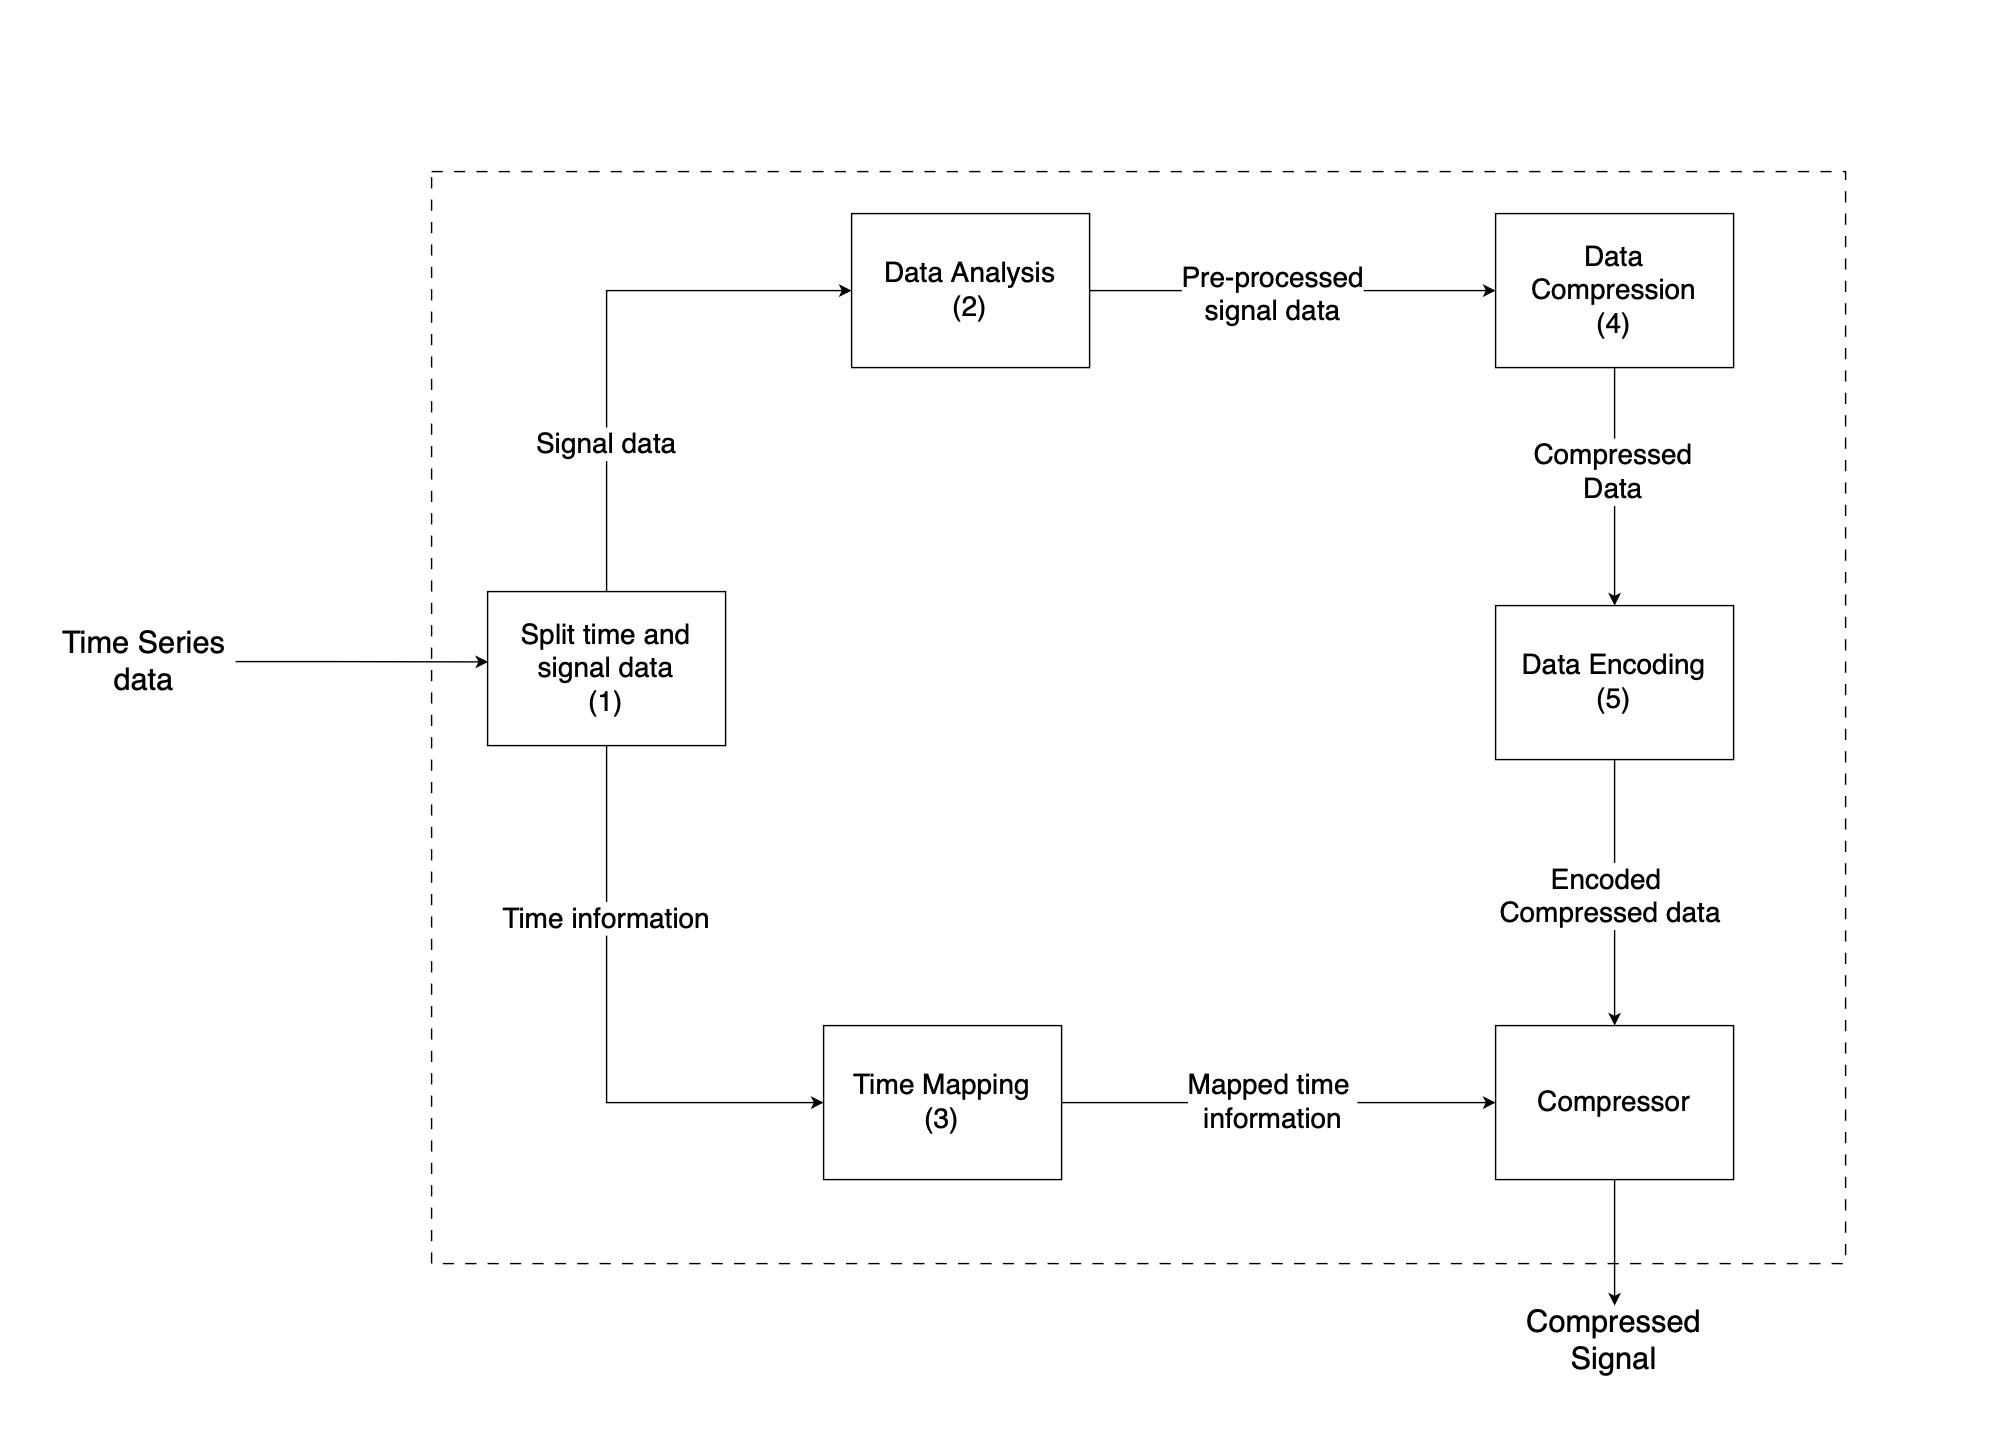
\includegraphics[width=0.5\textwidth]{Fig2.png}
  \caption{Internal Diagram of the ATSC Compressor stage}
  \label{internal}
\end{figure}

\subsection{ATSC Compressor}

\subsubsection{Split time and signal data}
First part of the processing is to split the signal into is two components, time and the signal.

\subsubsection{Data Analysis}
In this stage signal undergoes a statistical pre-processing, calculating the minimum, maximum, mean, variance, etc.
Also, the splitting of the signal into different blocks is performed here.
The block sizes are dynamic, and the sizing is done via 2 methods, either a discrete wavelet transform (DWT)\ref{wavelet} or sizing for optimal FFT processing (in the form of $slice = 2^n * 3^m$).
Given the computational cost of DWT, smaller signals are immediately sliced for FFT optimal size. In the other cases, DWT is performed first and if there is no high frequency components detected for slicing, FFT sizing is then performed.
This information is provided to the Data Compression stage along with the signal data.

\begin{figure}[ht]
  \centering
  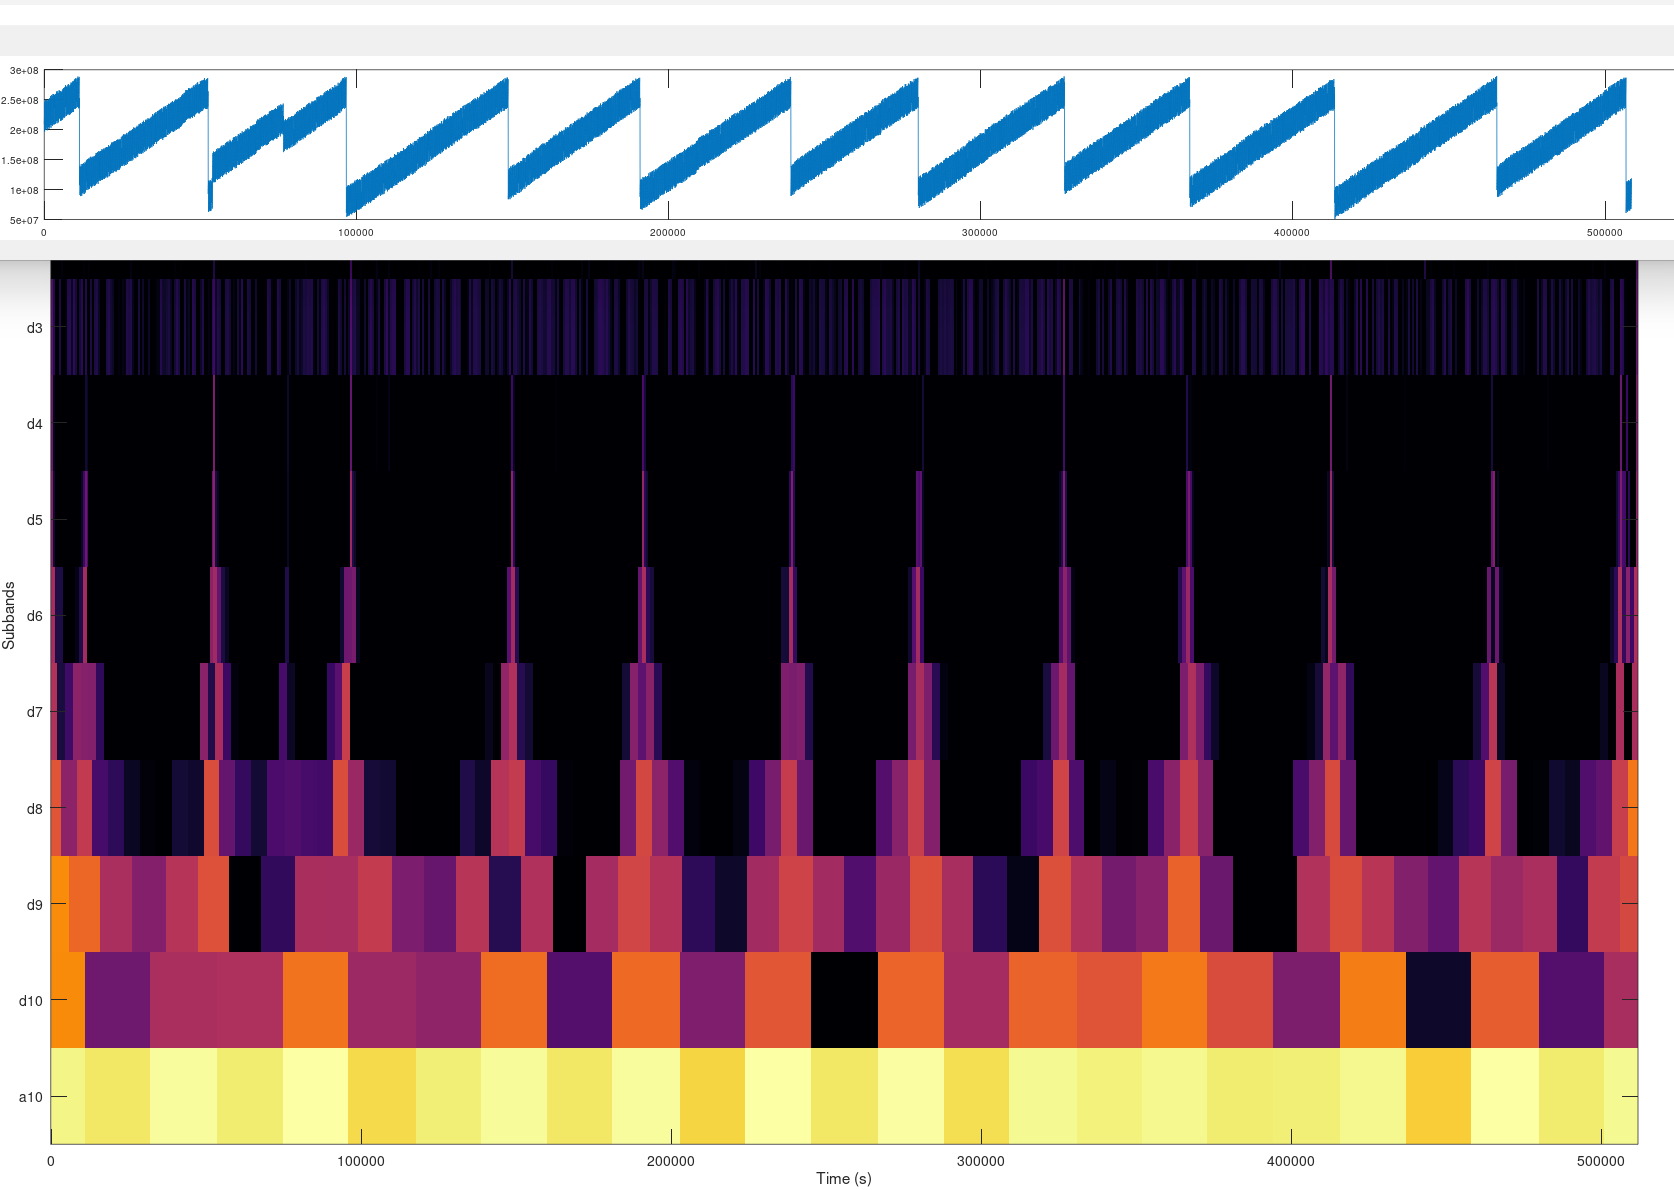
\includegraphics[width=0.5\textwidth]{wavelet_heap.png}
  \caption{Example of wavelet detection of high frequency sections to slice the signal. Signal on top and Wavelet Analysis on bottom.}
  \label{wavelet}
\end{figure}

\subsection{Time Mapping}
To facilitate precise access to samples without the need for full file seeking or decompression of the full file, ATSC generates an index. This index ensures efficient retrieval of relevant portions of the signal, a critical aspect in the decompression and streaming processes.
The indexing technique is further explained in his own section.

\subsubsection{Data Compression}
The signal samples are divided into blocks, and for each block, ATSC applies modelling techniques tailored to the specific characteristics of the signal. 
This may involve techniques such as Linear Predictive Coding (LPC), Polynomial Prediction, Fast Fourier Transforms (FFT), or other methodologies that best suit the signal's behavior. 
For a special case of signals that are continuous only a single value is stored, alongside the number of samples.
This modeling converts the original samples into an approximated formula.
Error correction and artifact reduction are also performed at this stage.
In some cases it is possible to match the original signal precisely and no other data is stored, otherwise an array of values representing the biggest outliers are stored alongside the formula type and its components.
This leads to a high number of data points being converted into a mathematical formula and its components.
A deeper dive into this is done in the Compression\ref{section:compression} section of this study.

\subsubsection{Data Encoding}
The last step of optimization is done by reducing the information to the minimal computational size needed for each sample. 
Samples are normally provided in 64bits size, this step can reduce the sample size to 8bit or any other size that the samples fit.

\subsubsection{Compressor stage}
This is the final stage, it just joins the compressed data alongside the index.

\subsection{ATSC Decompressor}

The decompression stage is fairly simple compared to the compressor.
This allows a faster decompression, a prerequisite for a successful implementation.
A decompression can be done for a full file, or for a specific segment of the file.
The basic principle of operation is the following:
\begin{itemize}
\item{\textbf{\textit{Identifying the Samples to be Retrieved:}}} Either all or a specific segment, the header of the file is read to find the block locations.
\item{\textbf{\textit{Data Retrieval Using the Index:}}} Check the index to identify in which blocks the samples are. In case of all the samples this step is ignored.
\item{\textbf{\textit{Sample decompression:}}} Once the relevant data segment is identified, ATSC initiates the decompression of the data.
For the located data samples, the block information is retrieved, the correspondent formula and its parameters are used to construct the representation for the sample interval. Any error correction is also applied.
\item{\textbf{\textit{Timestamp Integration Post-Decompression:}}} Following decompression, the samples, now in their extracted form, receive timestamp information from the index. This final step ensures temporal accuracy and relevance of the retrieved data.
\item{\textbf{\textit{Streaming/Writing data out:}}} Under a streaming process, samples are sent while being decompressed. ATSC also supports full file decompression where all the data is decompressed and then send out, or written out to an output file.
\end{itemize}

\section{Compression Methods}\label{section:compression}

Most of the work is done in this step. 
After a statistical analysis the signal, the compressor stage decides which approach is best for a given block of samples.
Alternatively, a small subset of the block (128 samples) is compressed using all available compressors and the best one is selected.
Depending on the error allowed for the compression, a less optimal method might be selected trading off precision for space savings. 
Each compressed block header always have the following information:

\begin{itemize}
    \item Compressor used - 1 Byte,
    \item Minimum and Maximum value in the block - 4 Bytes each,
    \item Compressor parameters (e.g. FFT frequencies) - Variable,
    \item Error correction points - Variable;
\end{itemize}
\vspace{5pt}

\subsubsection{Fast Fourier Transforms (FFT)}

Compression with FFT is done via a conversion of the signal to the frequency domain. Once in the frequency domain, we store a subset of frequencies.
The number of frequencies selected depends on the error margin we want to store the signal with. Since the signals are always real, the worst case scenario (lossless compression) half the frequencies need to be stored.
But since every frequency is represented by a pair of (Real, Imaginary) values, the lossless compression is next to none. 
The frequency pairs are always represented by two floats, either 32 or 64 bits depending on the precision required.
In a lossy scenario, and depending on the signal, 10x reduction in size is easily achievable within a 1\% to 3\% error margin.
To decompress, the Inverse FFT is applied on the available frequencies, zeroing out the missing frequencies.

\begin{figure}[ht]
  \centering
  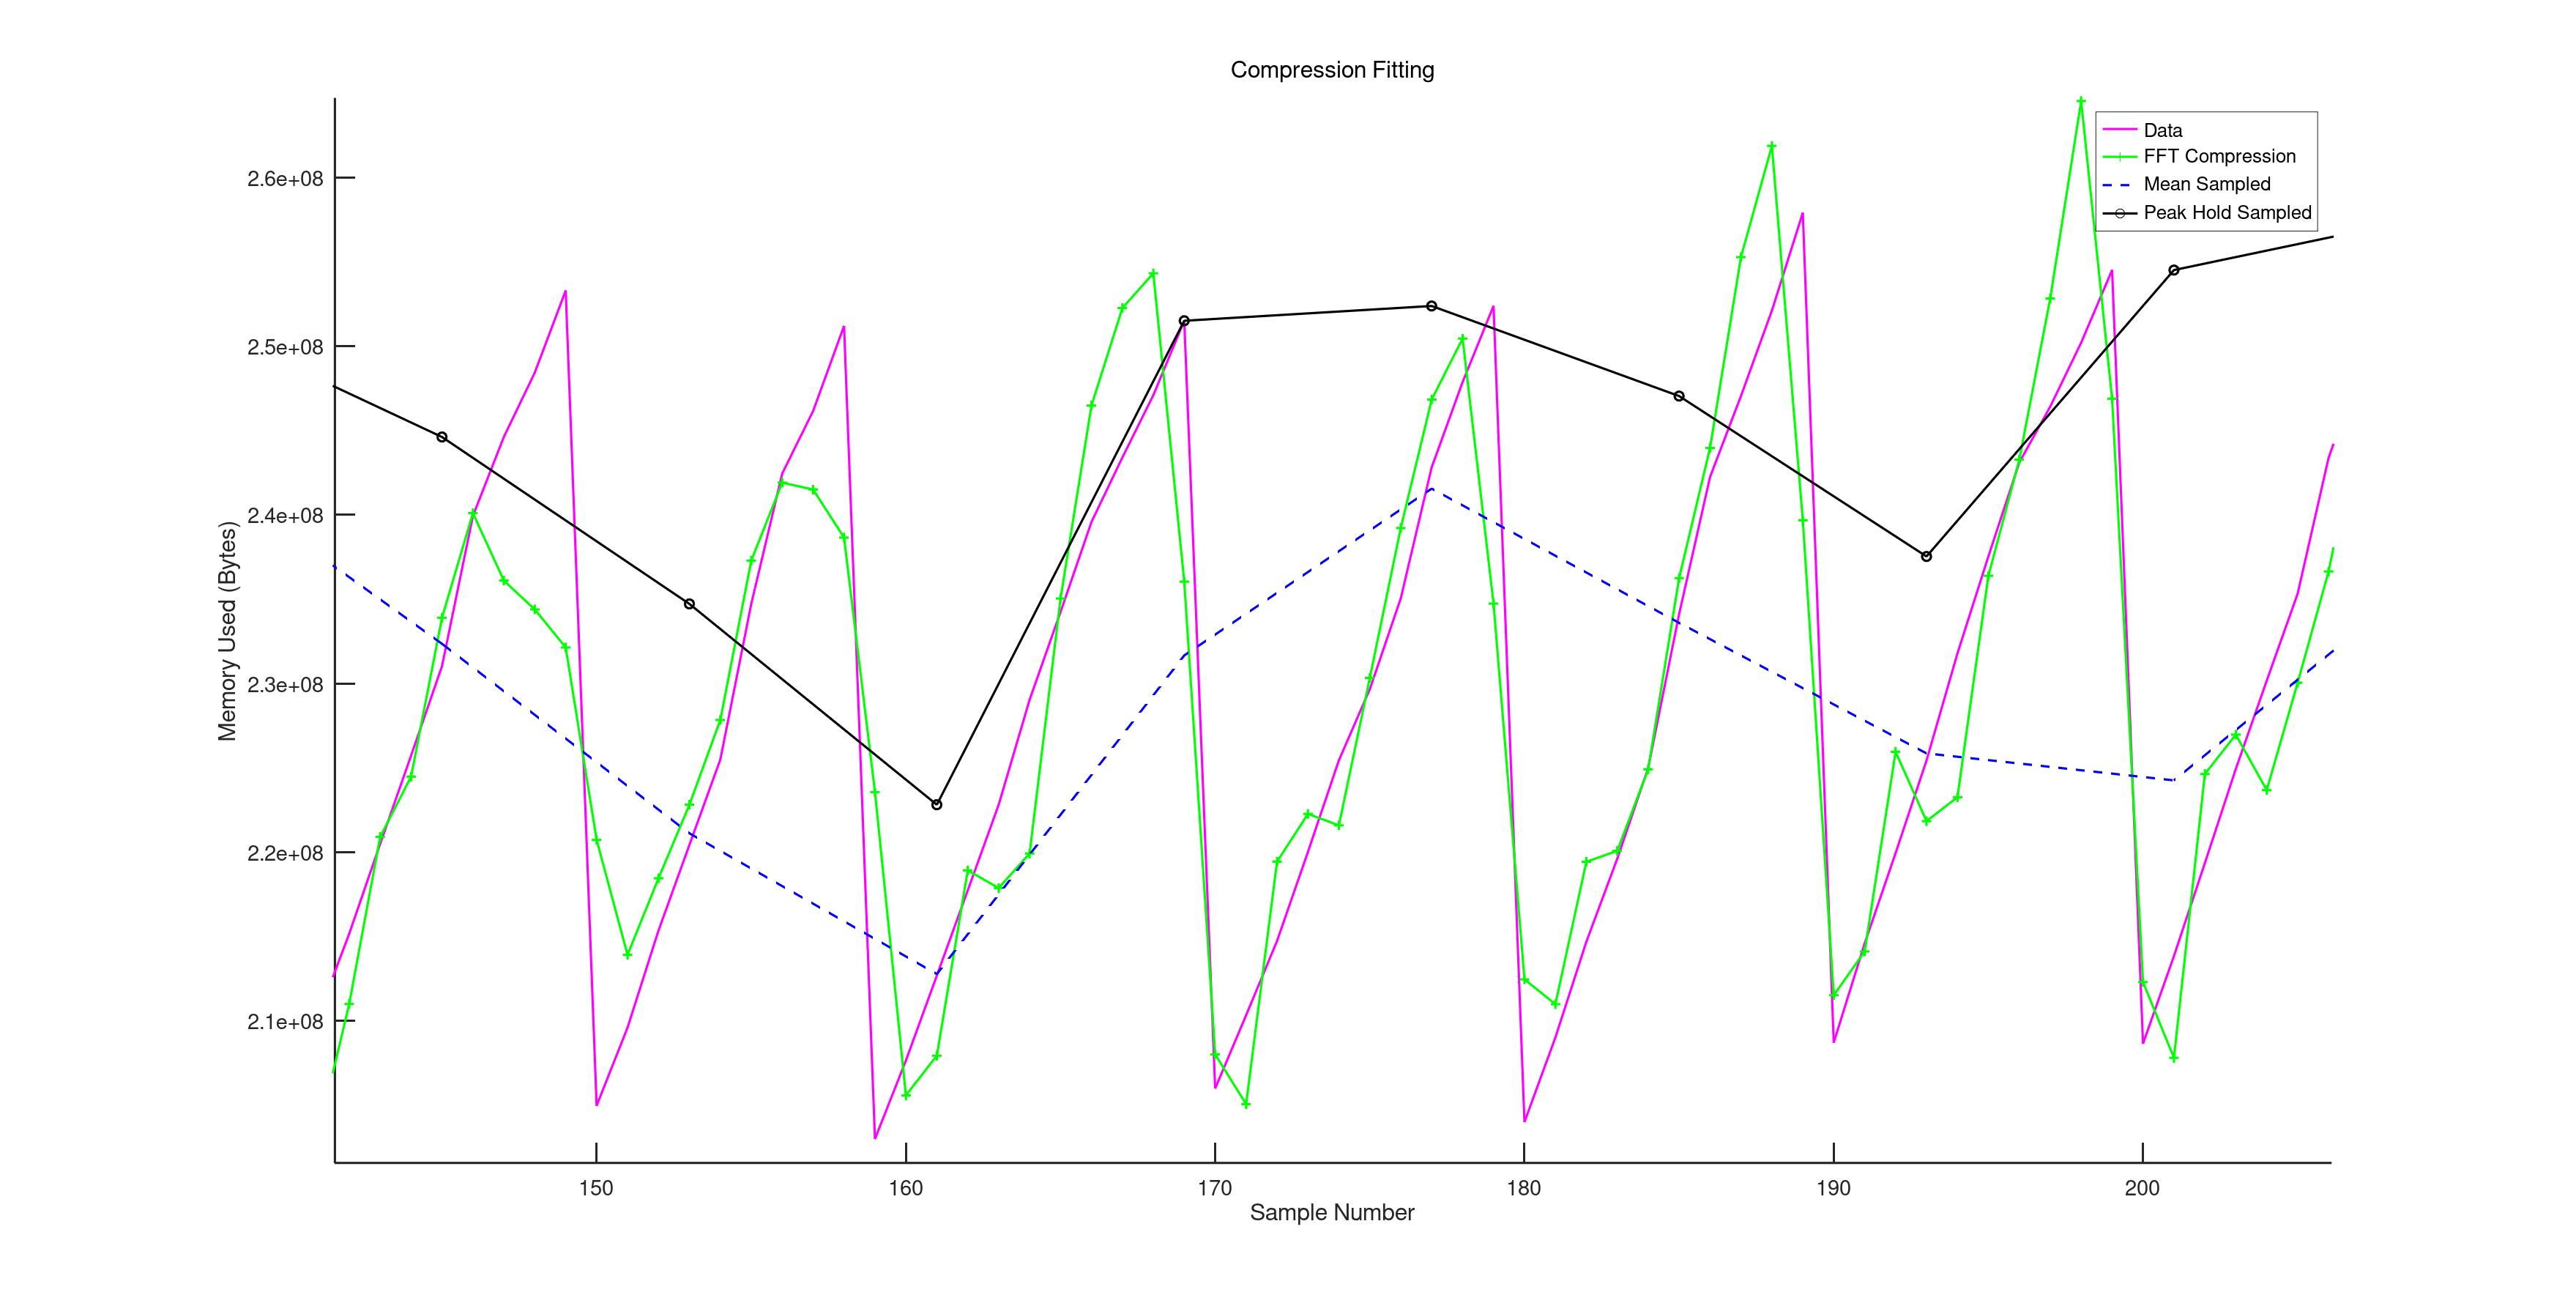
\includegraphics[width=0.5\textwidth]{fftvsaverages-2.png}
  \caption{Signal Fitting of the original data vs FFT Compression, Average Sampled and Peak Hold at the same compression ratio (8x).}
  \label{fft_comparison}
\end{figure}

\subsubsection{Spline Interpolation}

Another compression method is via a Spline Interpolation. 
For this study, we mixed Linear interpolation with Catmull-Rom interpolation, linear until we have enough data for a Catmull-Rom, and then we proceed with Catmull-Rom for the remaining of the signal.
The method is similar to the FFT, where several points are stored, and the corresponding outputs calculated via Spline Interpolation.
Once a Spline is generated within the margin of error provided, the points that generated that spline are stored.
An advantage of Spline Interpolation vs FFT is that the FFT always need to store the data as a pair of floats. 
While the Spline Interpolation the points are the same as the data points, so a integer signal would be stored as integer with the same bit depth as the original signal.
This could be something as small as 8bit per point.
In the decompression process, we do the interpolation calculation and retrieve the points requested.
No need even to calculate the whole spline, only the segments corresponding to the samples.

\subsubsection{Multivariate Interpolation}

In an almost identical process to the Spline Interpolation, we used Inverse Distance Weighting as a method to approximate the signal.
The results are solid, but almost the same as the spline interpolation, with the downside of a much slower decompression due to the complexity of the calculations.
Since the approach is very similar, the results were very easy to compare, and in most of the cases the Spline Interpolation offers the same compression this method is used only in very rare cases.
The similarity of the two also makes it difficult to choose each one to pick in a given scenario, and given the already mentioned disadvantages, this is only used in a manual selection of compressor methods.

\subsubsection{Linear predictive coding (LPC)}

A lot of lessons were learned from initial experiments with Audio compressors (mostly FLAC encoder).
Good results were obtained, and it was a natural approach to include the those within the available compressors.
The approach is exactly the same as described in the FLAC format [11], but with a small change.
The FLAC expects all samples to be integer, as such, floating point signals are discarded and not usable by definition.
But for signals with a very small precision and bounded (e.g. 0.00 - 100.00) we can convert those to integer and use the LPC compressor.
In practical testing, LPC offers the worst compression, worse than FFTs, so FFT is widely used, and in a similar case as the Inverse Distance Weighting, LPC is mostly relegated to a manual selection.
The only case where LPC is used, is in lossless compression, where it offers compression averaging between 2x to 8x.

\section{Artifact Detection and Correction}

All the methods described above generate almost always, a lossy compression. 
But sometimes, the methods above might generate artifacts that remove quality, or might provide wrong information to a viewer of the signal\ref{fig:artifact}.
Those artifacts are points that are generated from the mathematical approximations and are far from the original data points.
They constitute point errors bigger than any other points in the generated data.

\begin{figure}[ht]
  \centering
  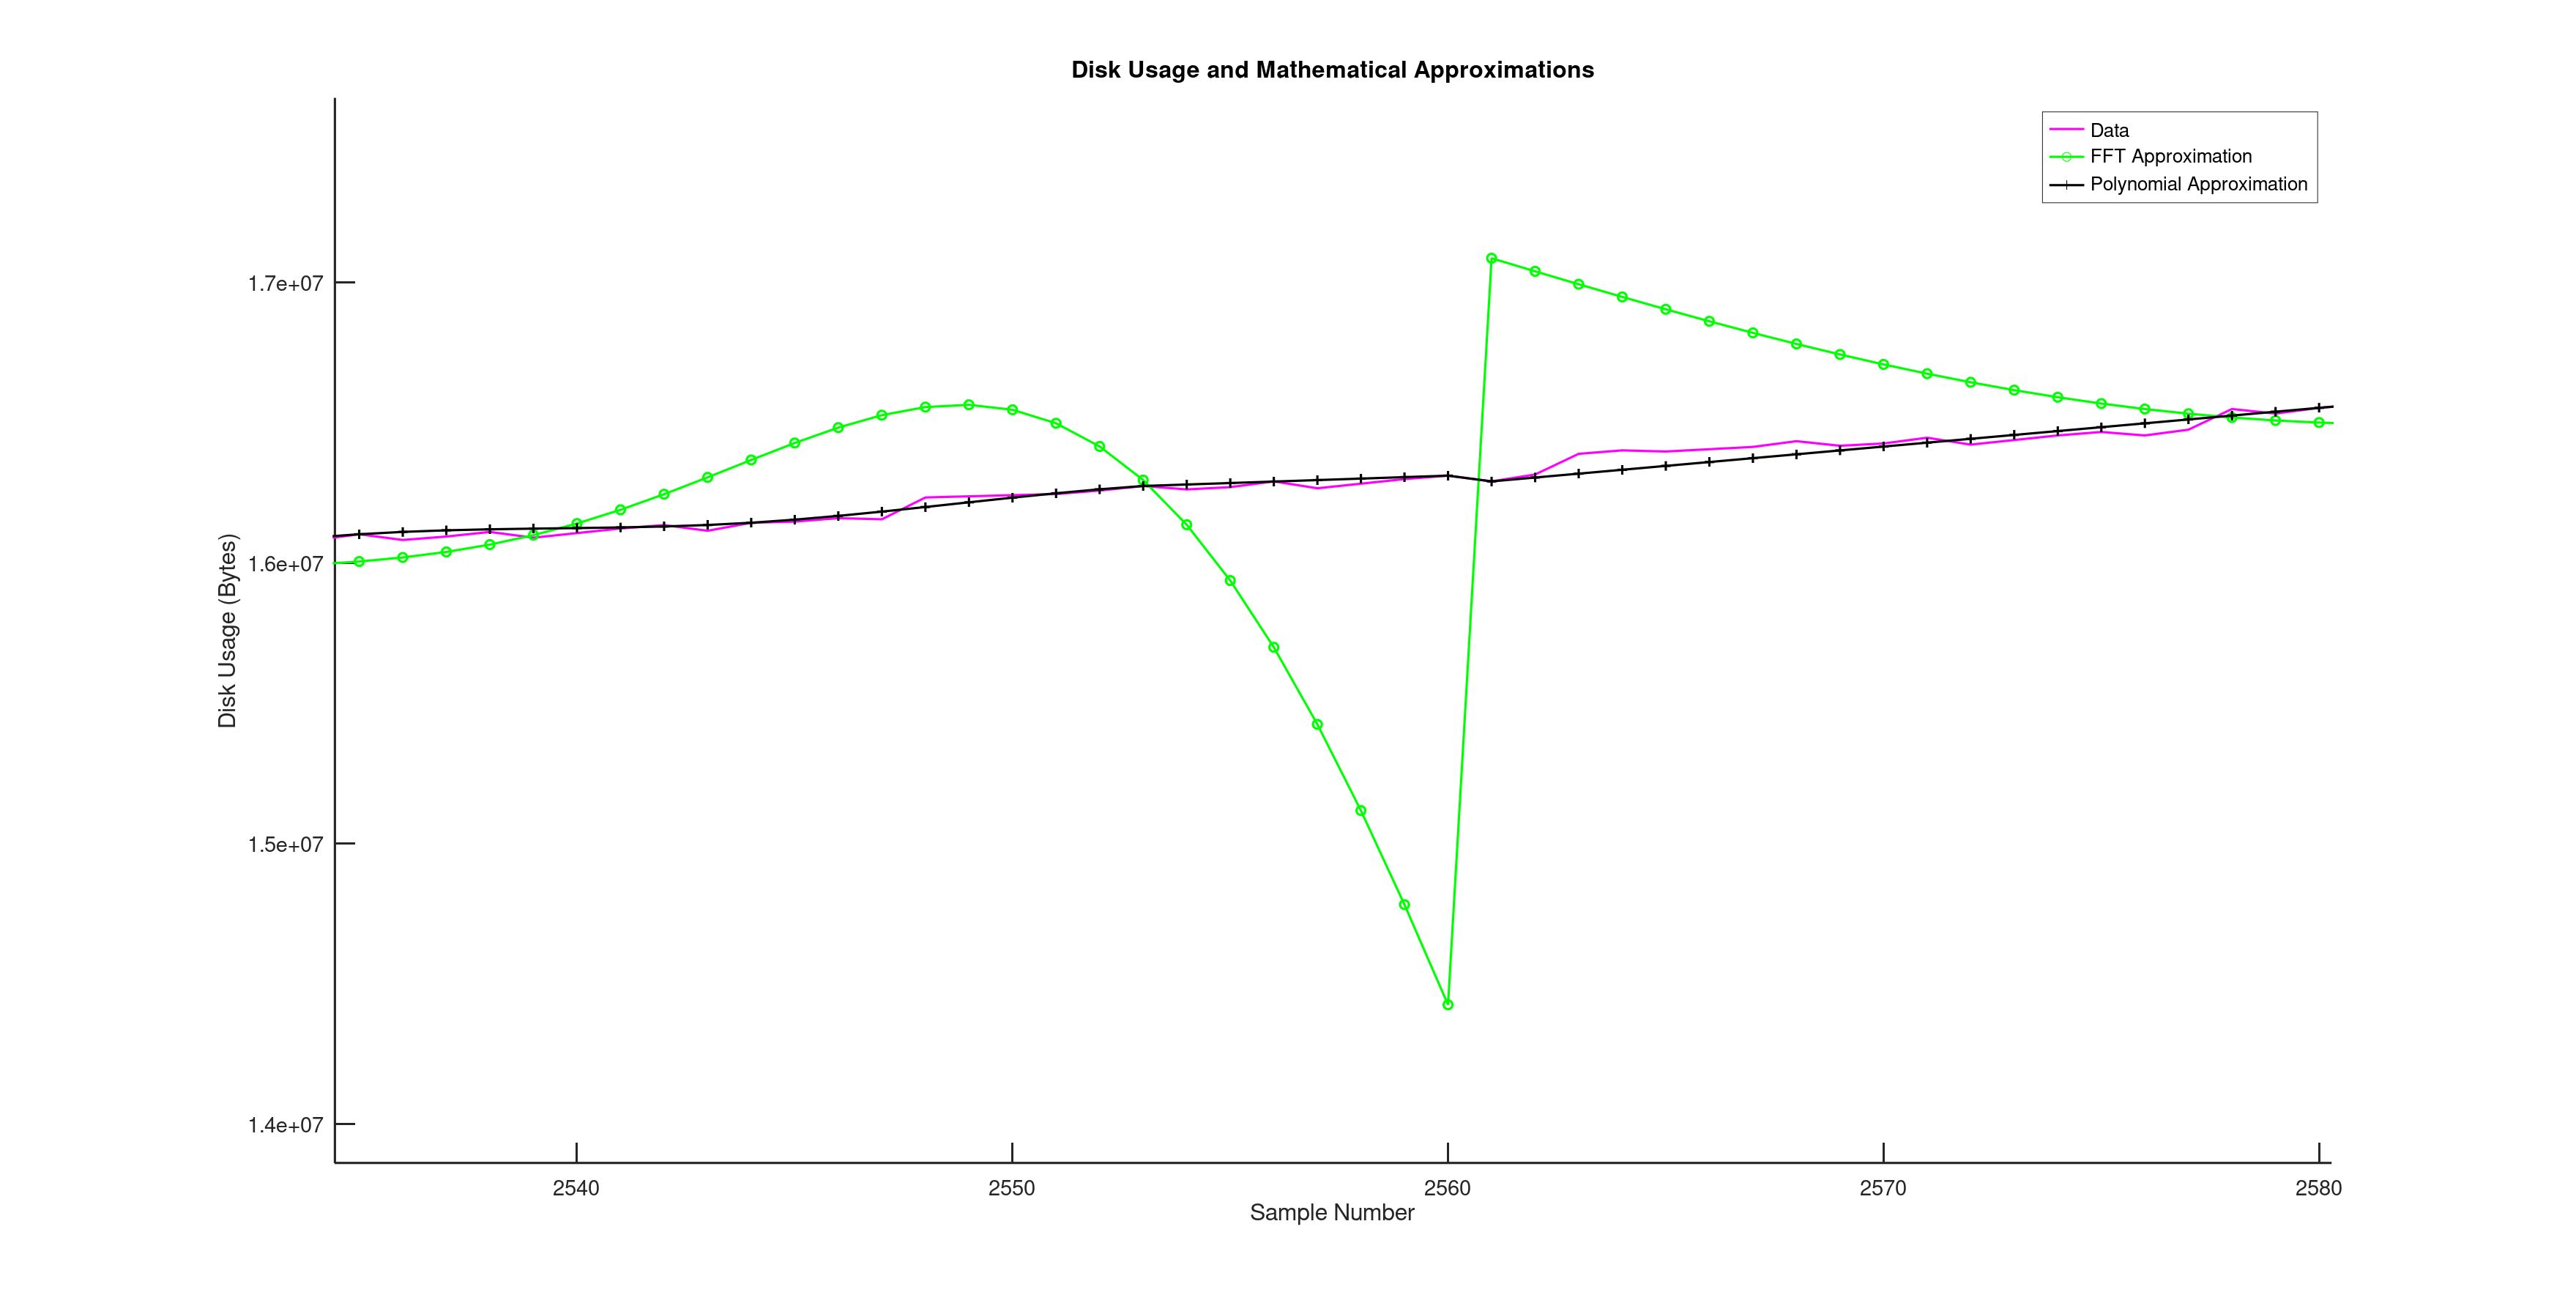
\includegraphics[width=0.5\textwidth]{artifact-2.png}
  \caption{Compression artifact from the FFT approximation.}
  \label{fig:artifact}
\end{figure}
\vspace{5pt}

For reducing the error of the compression and/or remove artifacts from the generated signals the following process is used:

\begin{itemize}
    \item Error detection via Mean Absolute Percentage;
    \item Storing of the errors that are above the defined error threshold;
    \item Store the location of the biggest errors and the correspondent original data point;
    \item When decompression happens, replace the generated points by the stored data.
\end{itemize}

This approach not only removes the biggest artifacts from the data, it also lowers the error rate of the signal.
On a good fitting, we can avoid storing any point, so the importance of the fitting.
A tradeoff exists, since a better fitting need more data stored (e.g. More frequencies for FFT), and storing errors need space.
For lossless compression all the point differences need to be stored.
In a lot of cases this leads to almost no compression unless the signal has a perfect fitting with the mathematical representation.

\section{Indexing Samples with VRSI (Variable Rate Sampling Interval)}
\subsubsection{Overview of VRSI Mechanism}

In the methodology section, a critical aspect of the process involves indexing samples for efficient data retrieval. Variable Rate Sampling Interval (VRSI) is employed to manage the sampling intervals effectively. VRSI operates on the premise that samples occur at evenly spaced intervals, such as every 5 seconds, 20 seconds, or 60 seconds.
\vspace{5pt}
\subsubsection{Line Segment Representation}

For each sampling interval, a line segment is created with specific fields:

\begin{itemize}
    \item \textbf{Start Timestamp:} The timestamp marking the beginning of the sampling interval.
    \item \textbf{Sample Interval:} The time gap between consecutive samples.
    \item \textbf{Starting Sample:} The index of the first sample within the segment.
    \item \textbf{Number of Samples:} The total number of samples within the segment.
\end{itemize}
\vspace{5pt}
\subsubsection{File Structure}

These line segments are then stored in a file, accompanied by the lowest and highest timestamps in the segments represented. This file structure allows for easy identification of whether a requested interval is present in the index. If the requested interval falls entirely outside the timestamps in the file header, no samples are available for that interval.
\vspace{5pt}
\subsubsection{Handling Temporal Gaps}

In cases where a metric stops reporting for a period, a new line segment is generated, ensuring accurate representation of the sampled data over time.
\vspace{5pt}
\subsubsection{Example VRSI File Content}

\begin{verbatim}
55745
59435
15,0,55745,166
15,166,58505,63
\end{verbatim}


\begin{itemize}
    \item Line 1) Represents the first timestamp.
    \item Line 2) Represents the last timestamp.
    \item Line segments are detailed below:
    \begin{itemize}
        \item The first line segment has one sample every 15 seconds, starting at timestamp 55745, with a total of 166 samples.
        \item The second line segment also has one sample every 15 seconds, starting at timestamp 58505, with 63 samples.
    \end{itemize}
\end{itemize}
\vspace{5pt}
\subsubsection{Locating Samples (Read Path)}

In the read path, when locating a sample in a file using the index, timestamps or timestamp ranges are specified (e.g., "All the samples from 3:30 PM to 4:30 PM"). The system checks if the requested timestamps are within the available timestamps in the file header. If found, the sequence of sample numbers is extracted, indicating the samples needed for decompression.
\vspace{5pt}
\subsubsection{Creating/Updating the Index (Write Path)}

When a new sample is added, the index is updated. Since time progresses linearly, and samples occur in sequence, the system only needs to:
\begin{itemize}
    \item Update the last segment's sample number or
    \item Create a new segment.
\end{itemize}

Existing segments are incremented if the sample timestamp is the next in sequence. If a segment does not exist or the timestamp is not the next in sequence for the latest segment, a new segment is created. This approach ensures an efficient and organized index for managing variable rate sampling intervals.

\section{Results}

A real-world testing methodology was employed to assess the efficiency and effectiveness of ATSC. The ATSC server was configured as both a read and write backend for a Prometheus\cite{prometheus} instance, establishing a practical and relevant testing environment. 
In turn, the Prometheus instance was connected to an Instaclustr internal production 57-node Cassandra\cite{cassandra} cluster with a Prometheus endpoint enabled. The data flow was then collected at the node level and sent to the Prometheus endpoint that would forward it to the ATSC server configured as previously stated.
The server ran for approximated 18 hours over a 2 day period. Samples were collected at 1 point every 20 seconds, resulting in 5432 samples per each signal for each node. A total of 14386 signals were processed.
We removed signals representing aggregations (e.g. histograms), reducing the total number of signal to 13950 and the total data size to  with a total data size of 606,294,900 bytes.
ATSC ran with automatic compressor selection and a maximum allowed error of 3\%.

\subsection{A Best-Case Scenario Analysis}

Before delving into the detailed results, it is essential to address the ATSC single scenario.
The best case scenario for ATSC is a dataset that fits perfectly with a mathematical model.
In such a case, even with a growing number of samples it is possible to store a massive amount of data represented by only the mathematical formula, the sample number, and the index. In these circumstances, compression ratios above 3000x were achieved.
This ideal scenario is also realistic, as stale or infrequently changing signals always exist.
In our production tests, approximately 13\% of the data falls into these categories.

\subsection{Data Overview}

\begin{table}
\centering
\begin{tblr}{
  hline{2} = {-}{},
}
\textbf{Method} & \textbf{Compressed size (bytes)} & \textbf{Compression Ratio}   \\
Prometheus                  & 454,778,552                      & 1.33 \\
LZ4                         & 141,347,821                      & 4.29 \\
ATSC                        & 14,276,544                       & 42.47                                    
\end{tblr}
\caption{Benchmark results of compression performances between different compression methods.}
\label{table:results}
\end{table}

The compression performance of ATSC was benchmarked against two state-of-the-art methods (Prometheus and LZ4). Results obtained in the compression tests are shown in Table \ref{table:results} and Figure \ref{fig:histogram}. Overall, ATSC performed substantially better, achieving a compression ratio over an order of magnitude than the other methods tested (Table \ref{table:results}).
The data overview in Table \ref{table:results} provides a performance reference, while compression statistics and signal counts measure  the efficiency of ATSC's compression strategies. 
The compression effectiveness was quantified using the average compression ratios and the compression histogram (figure \ref{fig:histogram}). 

\begin{figure}[ht]
  \centering
  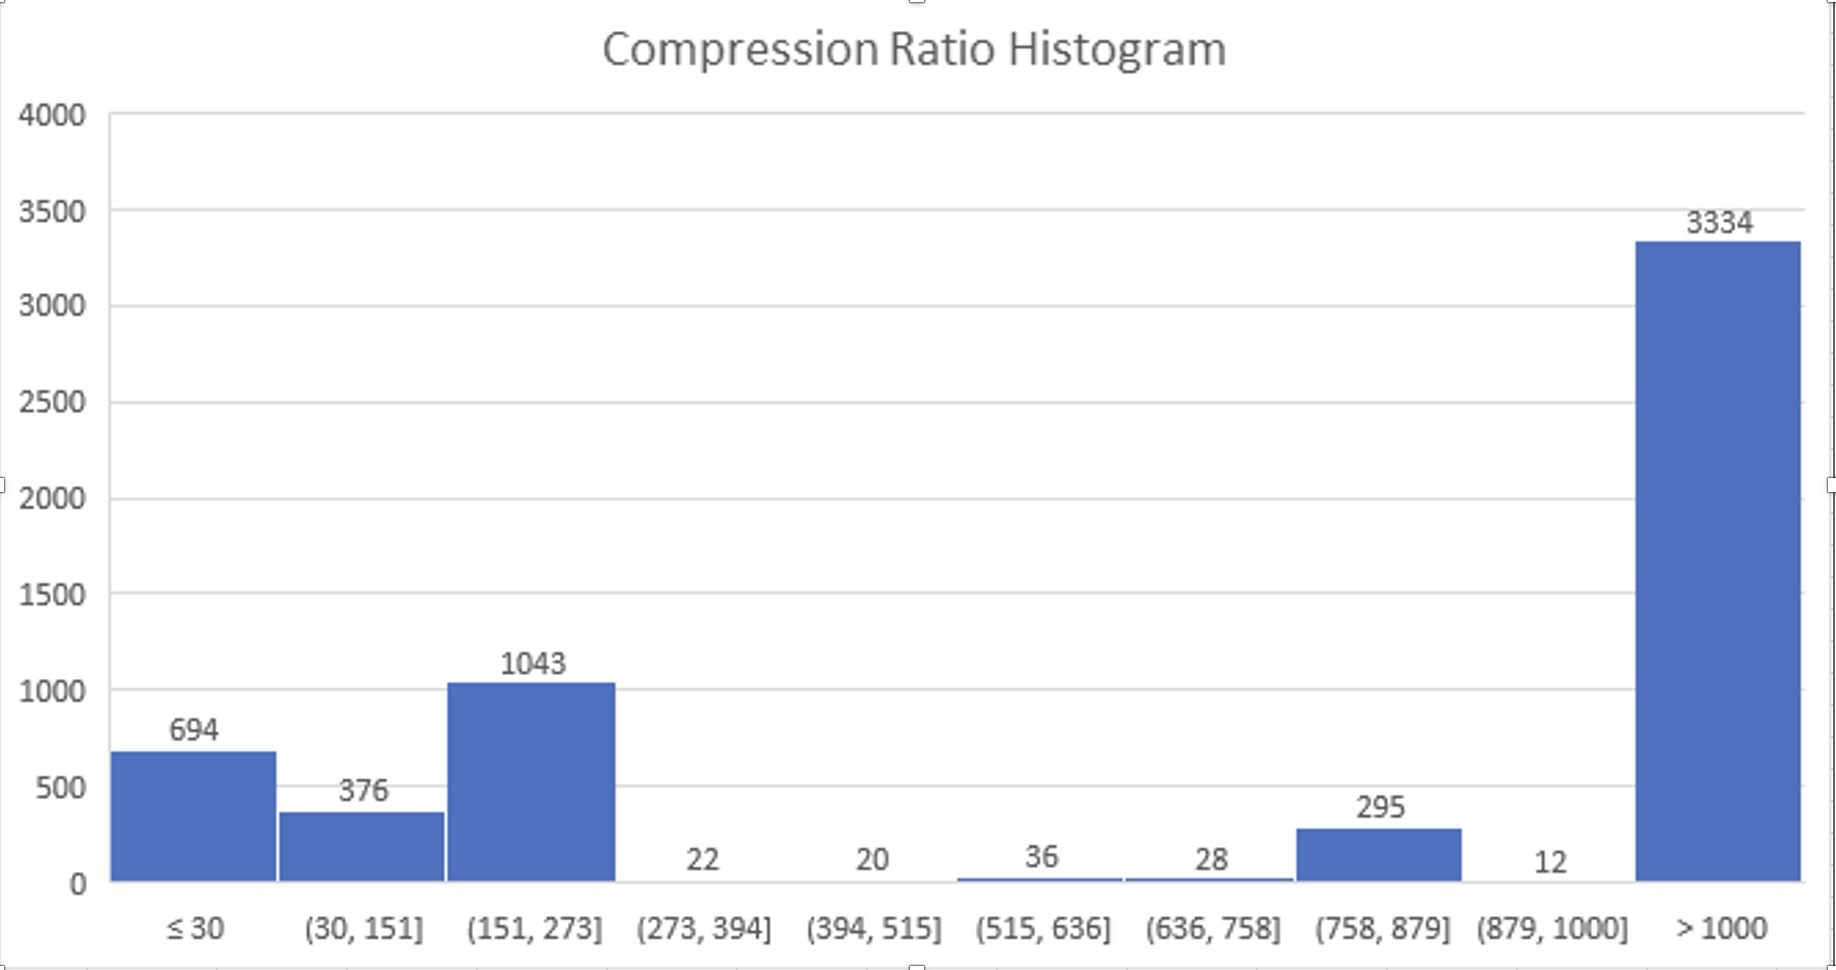
\includegraphics[width=0.5\textwidth]{Fig5.png}
  \caption{ATSC Compression Ratio Histogram}
  \label{fig:histogram}
\end{figure}
 
\subsection{Validation of results}

The previous results were validated by uncompressing the compressed data and comparing it with the original signal. The compressor chose to perform lossy compression, which was expected because it was set to automatically determine the best compression strategy and given a maximum allowed error. The degree of information loss varied for different signals but the overall performance was remarkable. For example, the mathematical approximations of “CPU usage” (Figure \ref{fig:cpu}) and “Disk usage” (Figure \ref{fig:disk}) were very close to the original data. The latter resulted in an error of less than 3\%. “Heap usage” is a signal that is normally very difficult to fit. Despite this, ATSC tracked the signal with an accuracy that was sufficient to capture the information.
As stated before, reducing the compression ratio can lead to a better approximation. However, our tests on real data shows that this difference is not significant, this is demonstrated in figure \ref{fig:heap}. 

\begin{figure}[h]
  \centering
  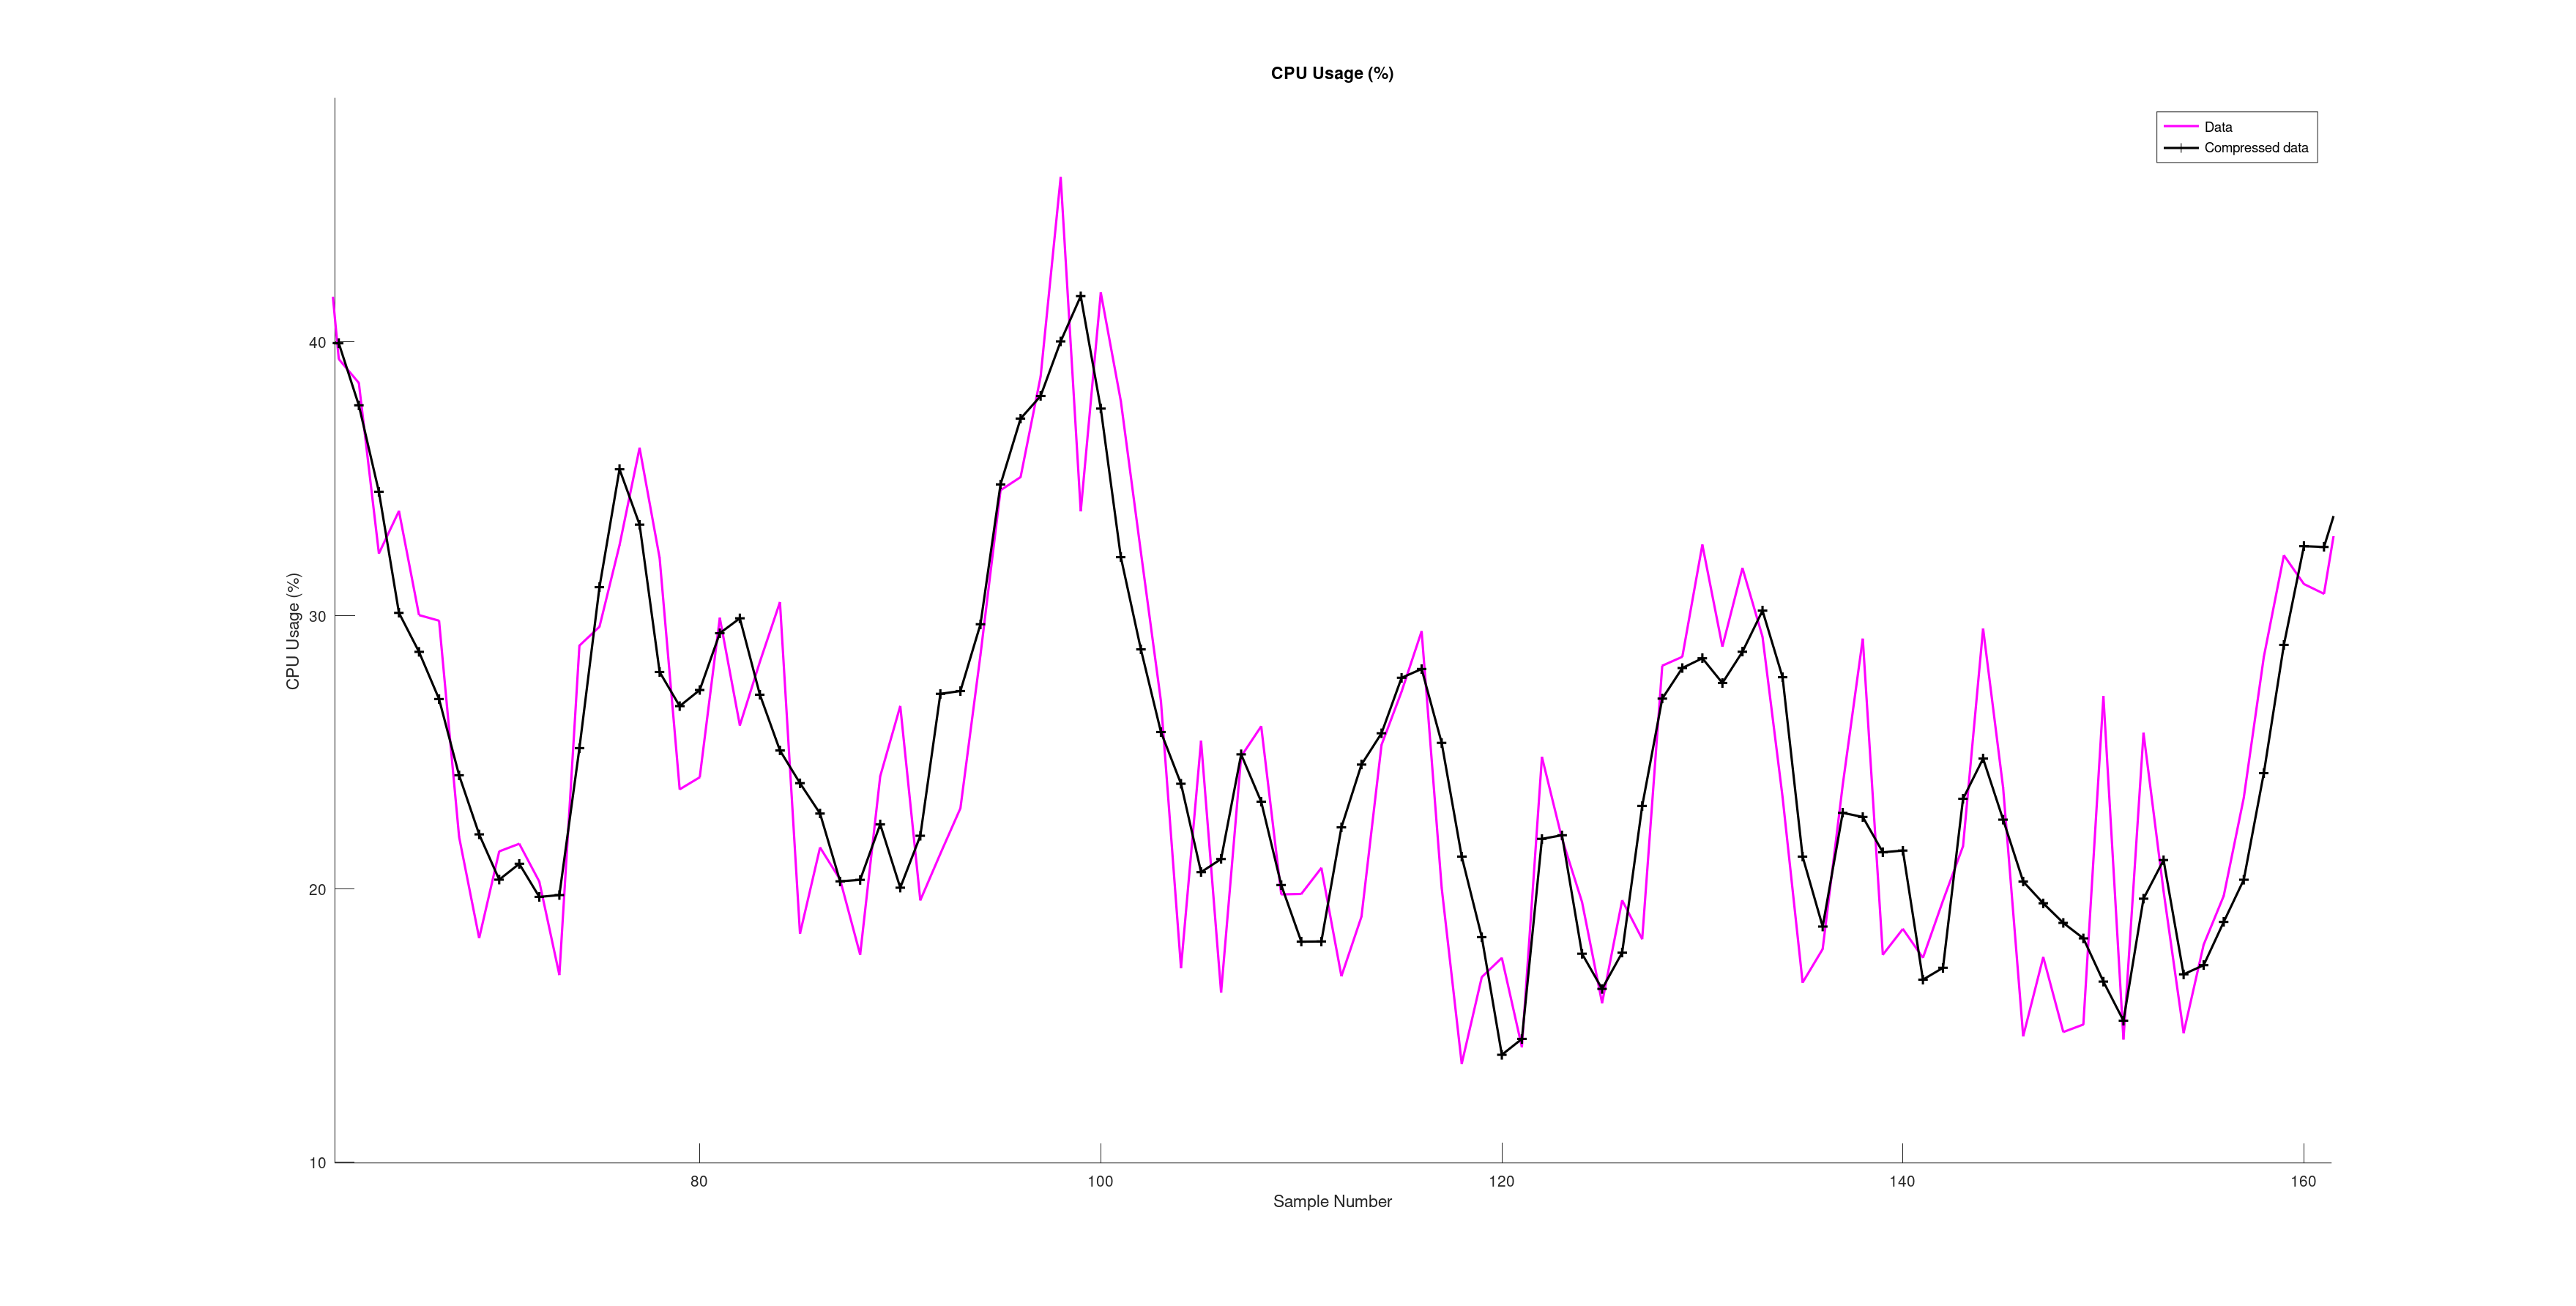
\includegraphics[width=0.5\textwidth]{cpu-usage-validation-2.png}
  \caption{CPU compression (17x) vs Original data}
  \label{fig:cpu}
\end{figure}


\begin{figure}[h]
    \centering
    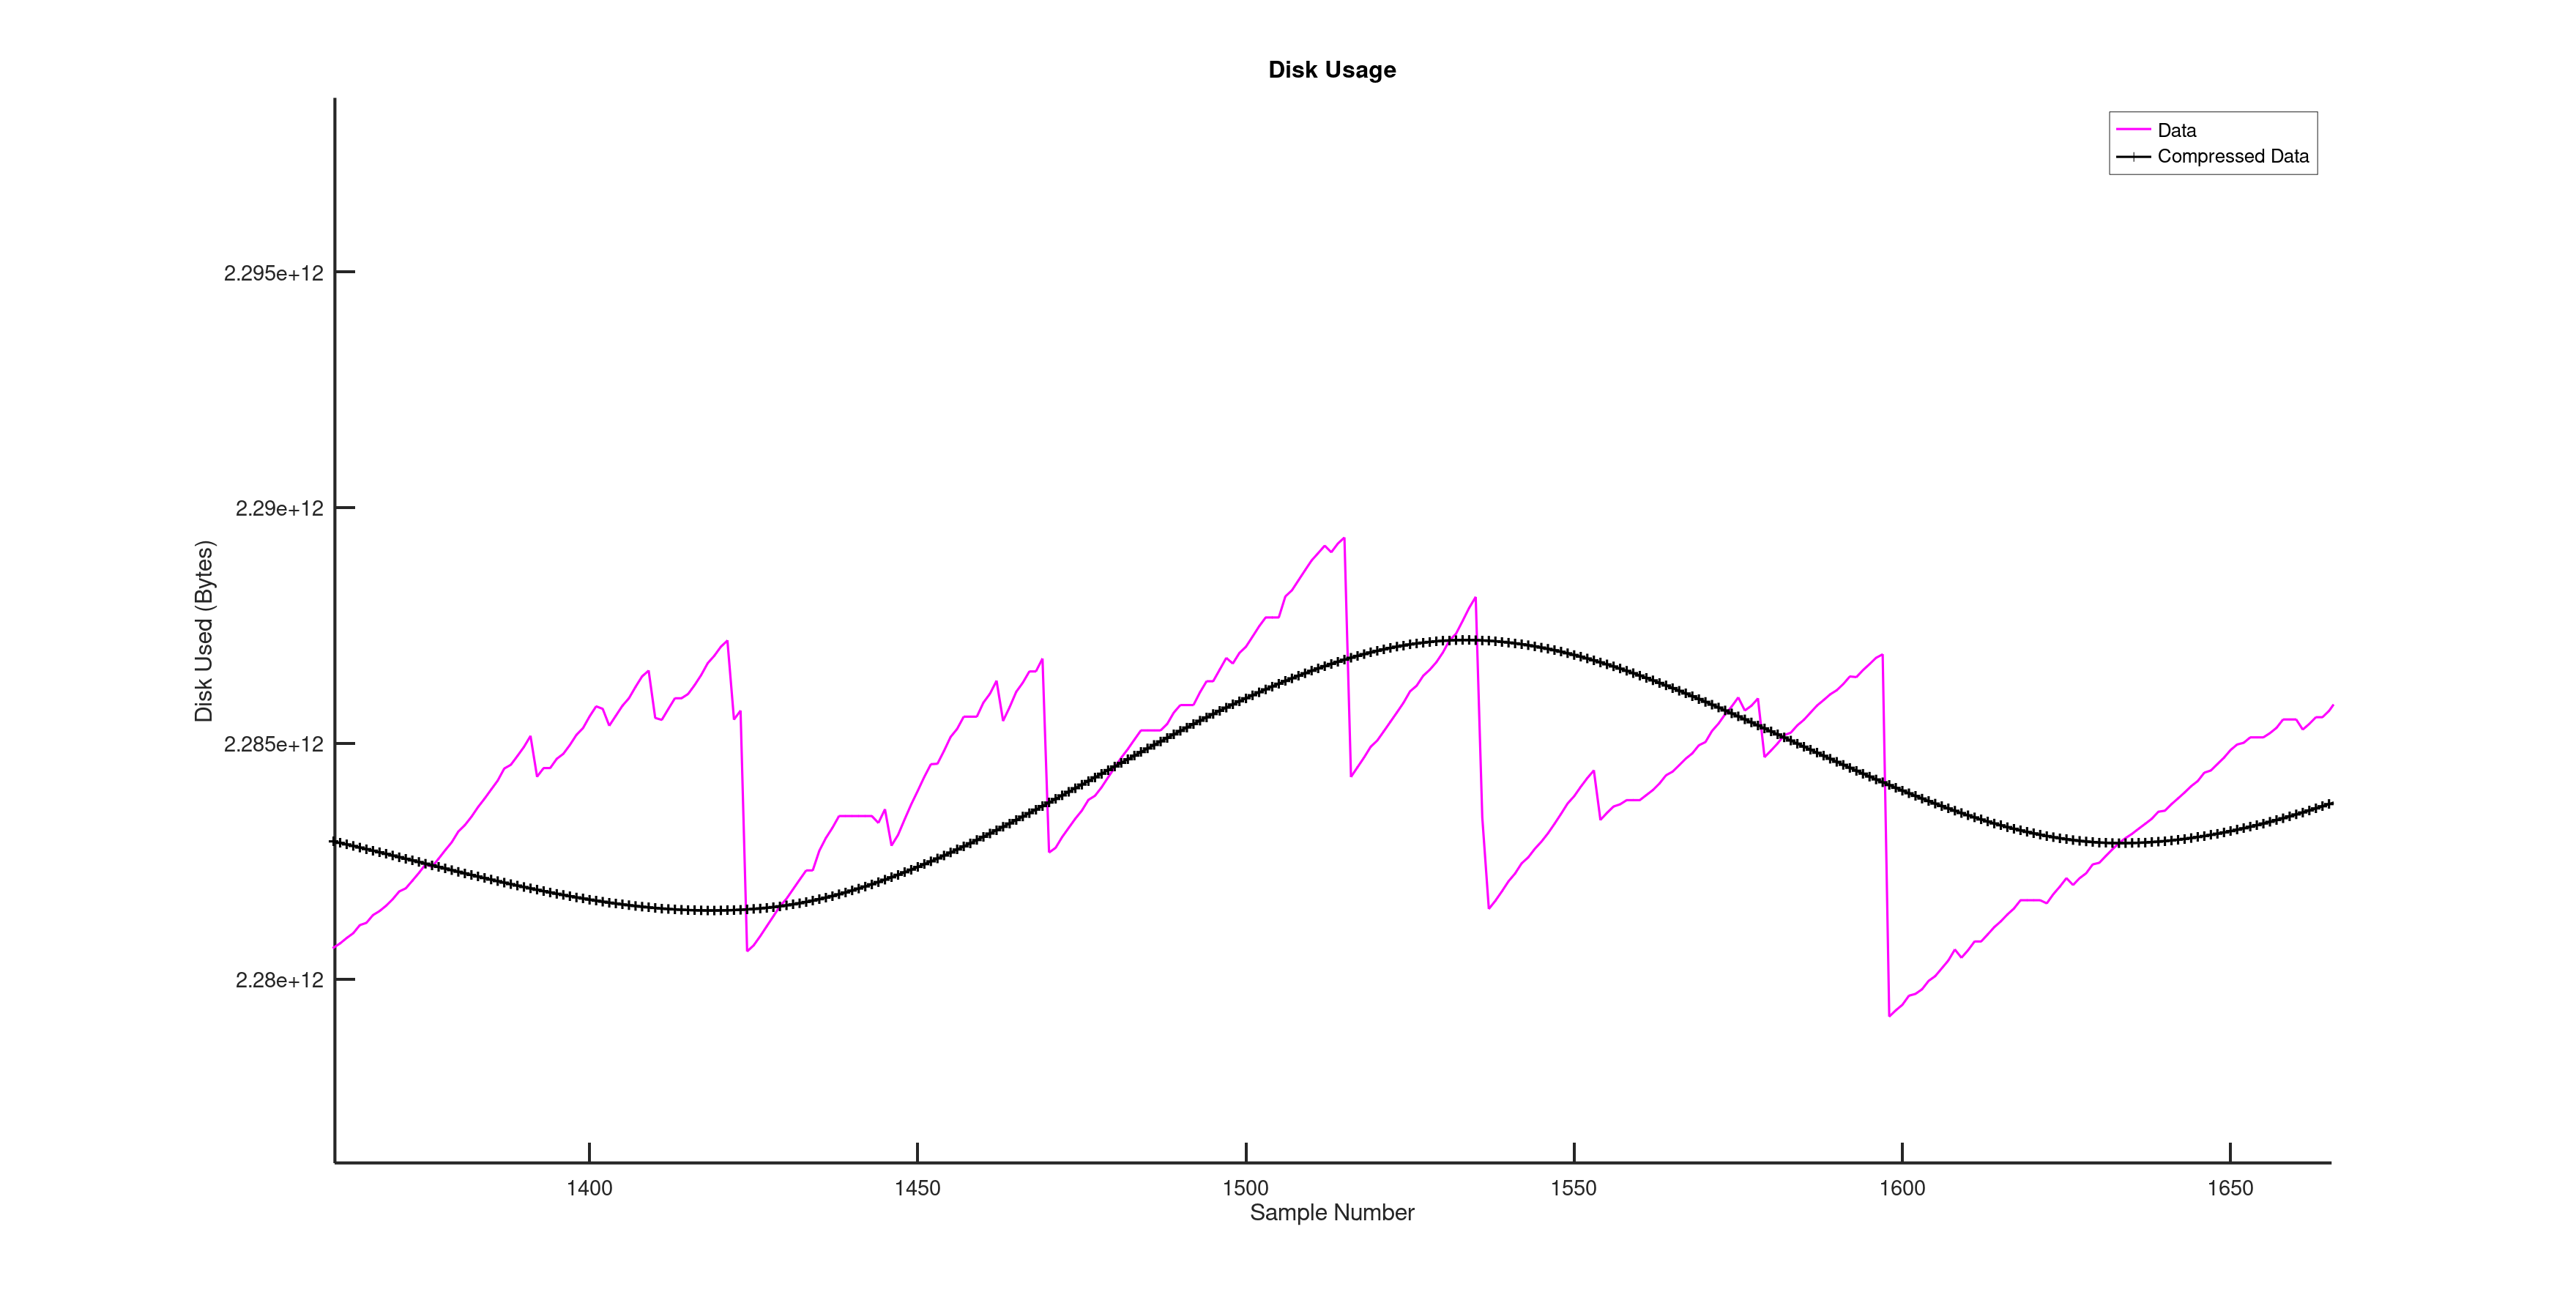
\includegraphics[width=0.5\textwidth]{disk-usage-validation-2.png}
    \caption{Disk compression (146x) vs Original data}
    \label{fig:disk}
  \end{figure}


  \begin{figure}[h]
    \centering
    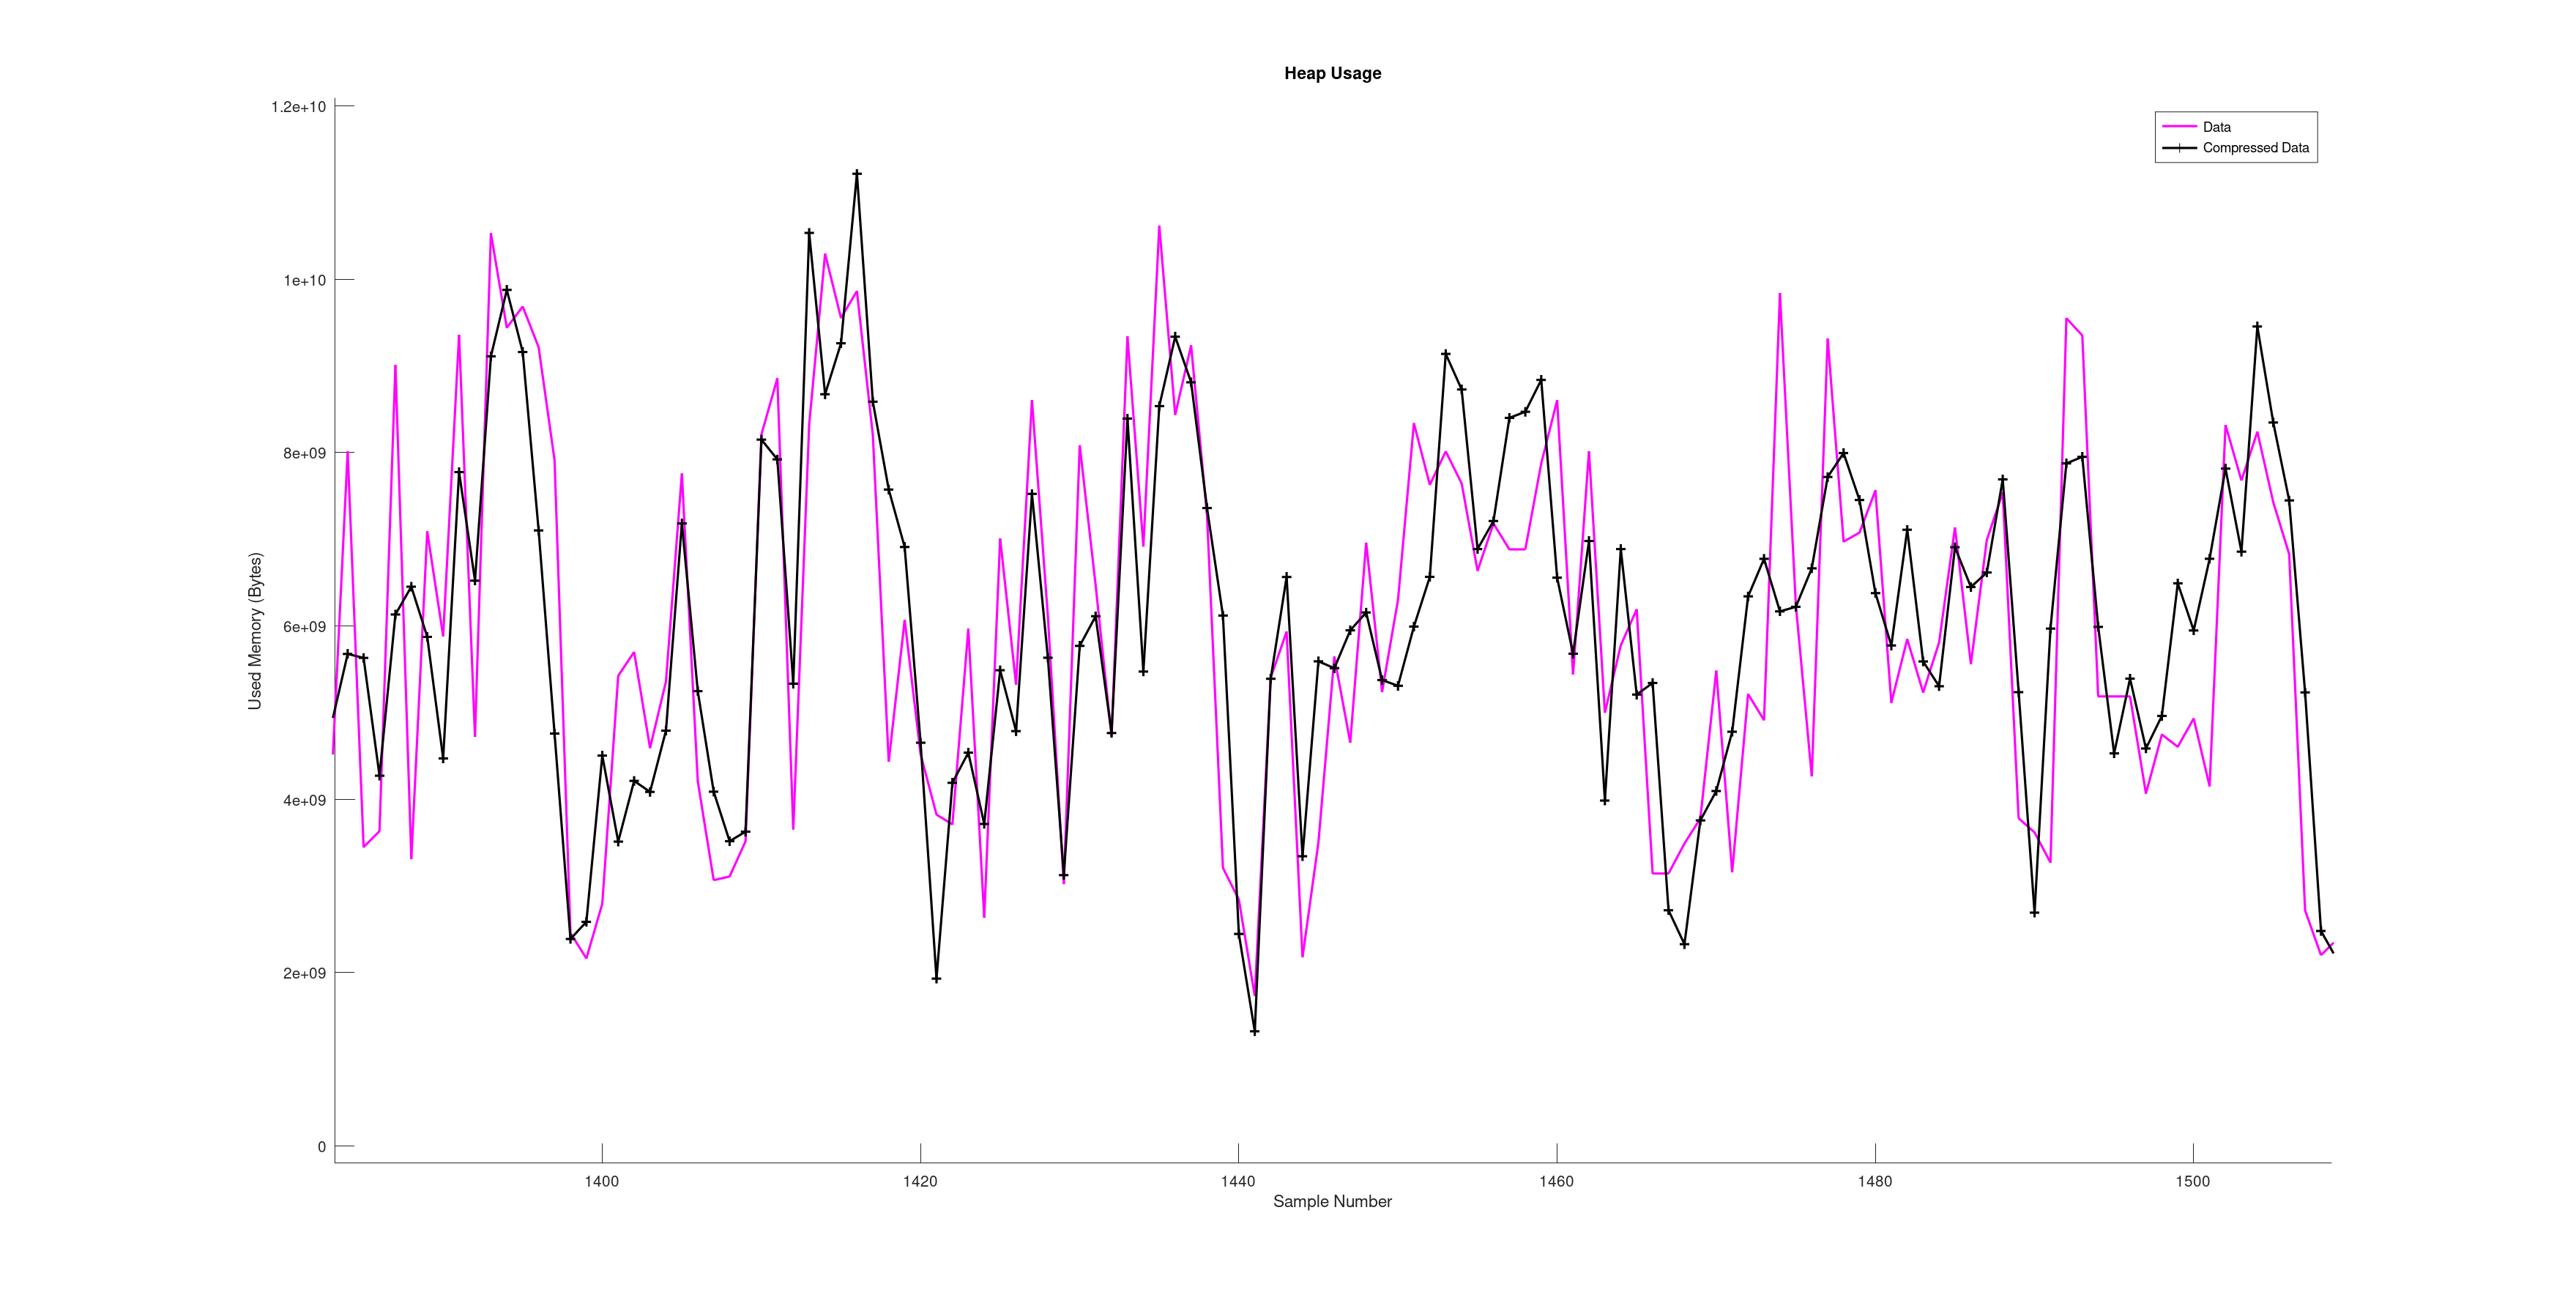
\includegraphics[width=0.5\textwidth]{heap-usage-validation-2.png}
    \caption{Heap Usage Compressed (18x) vs Original data}
    \label{fig:heap}
  \end{figure}
\vspace{10pt}


In conclusion, ATSC compression enabled compression ratios of approximately 60 times, achieving remarkable data reduction. 
These results substantiate ATSC's capabilities in optimizing storage space, offering valuable insights into its potential impact on real-world applications. 

\section{Future Work}

While ATSC shows a significant improvement over existing compression techniques for time-series,  several work directions can further expand its compression ratios, system integration, and others. 

\subsection{Compressor selection and optimization}

Currently, ATSC provides a small subset of fixed algorithms. The choice is made based on a simplistic statistical analysis. In the future, choosing the optimal algorithm for different datasets could be performed by an Artificial Intelligence (AI) model trained using a large number of signals. 
Or more robust and/or faster methods for 

\subsection*{Test further algorithms}

ATSC algorithm selection can be expanded alongside improved selection methods to further increase its achievable compression ratios.

\subsection{Integration with other systems}

While developing ATSC, we found that it creates similar outputs for many signals. This knowledge can be leveraged by having ATSC integrated in a database to identify such scenarios and avoid storing data once a specific output already exists. This would substantially improve space savings.

\subsection{Outlier Detection}

During our tests, we noted that the compression ratios for a given metric across all nodes would be mostly the same for systems with several nodes doing the same work (e.g., a Cassandra database with multiple nodes).
In some cases, we found that nodes had significant differences for some metrics, representing 2 to 10 times worse compression. na in-depth look into the detailed metrics showed that the node was misbehaving, having to be fixed 
or replaced. This ability to detect outliers by comparing compression is an application worth exploring.

\subsection{Use of Hardware Capacities}

Our approach yields savings in at-rest scenarios, as well as in transit and during compute processing. The ability to leverage client-side devices enables efficient processing and transport of monitoring data. Integration in system-on-a-Chip architectures could lead to further performance enhancements. This strategy positions our methodology at the forefront of efficient and resource-conscious computer systems monitoring.

\section{Conclusion}

In conclusion, the ATSC approach outlined in this study offers a novel solution for monitoring time-series data compression, particularly in computer systems. ATSC achieves impressive compression ratios, achieving over 1000x times compression. This innovative methodology addresses current storage and data transfer challenges.
\vspace{5pt}
Preliminary tests against a production cluster demonstrated significant space savings using ATSC compared to current state-of-the-art methods. This study emphasizes the importance of unique indexing for precise data retrieval, showcasing its efficiency in streaming and targeted decompression of relevant data segments.

The future work directions outlined underscore ATSC's commitment to continuous improvement, with a focus on automated selections, integration with time-series databases, and addition other capabilities. These efforts aim to keep ATSC at the forefront of efficient and intelligent time-series data compression.


\bibliographystyle{plain} % We choose the "plain" reference style
\bibliography{refs} % Entries are in the refs.bib file
\end{document}